\documentclass[tikz,border=10pt]{standalone}
\usepackage{pgfplots}
\pgfplotsset{compat=1.18}
\usepackage{amsmath,amssymb,bm}
\definecolor{darkbg}{HTML}{1a1a1a}
\definecolor{lightfg}{HTML}{e8e6e3}
\definecolor{accent}{HTML}{7cb87c}
\definecolor{accent2}{HTML}{6aa0b0}
\definecolor{mutedcol}{HTML}{9a9a9a}
\definecolor{bordercol}{HTML}{3d3d3d}
\definecolor{redcol}{HTML}{cc3333}
\definecolor{bluecol}{HTML}{4466cc}
\pagecolor{darkbg}
\color{lightfg}

\begin{document}
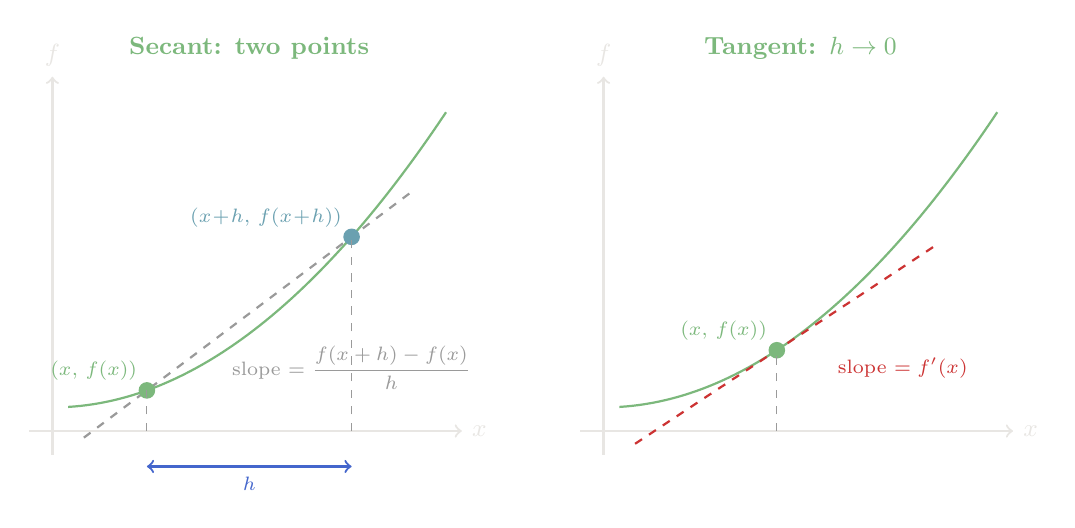
\begin{tikzpicture}

% --- Left panel: Secant ---
\begin{scope}[shift={(0,0)}]
  \node[anchor=south, accent, font=\bfseries\small] at (2.5,4.6) {Secant: two points};

  % Axes
  \draw[->, lightfg, thick] (-0.3,0) -- (5.2,0) node[right, font=\small] {$x$};
  \draw[->, lightfg, thick] (0,-0.3) -- (0,4.5) node[above, font=\small] {$f$};

  % Curve f(x) = 0.15x^2 + 0.3
  \draw[accent, thick, domain=0.2:5, samples=60] plot (\x, {0.15*\x*\x + 0.3});

  % Points
  \def\xa{1.2}
  \def\xb{3.8}
  \pgfmathsetmacro{\ya}{0.15*\xa*\xa + 0.3}
  \pgfmathsetmacro{\yb}{0.15*\xb*\xb + 0.3}

  % Secant line (extended)
  \pgfmathsetmacro{\slope}{(\yb - \ya) / (\xb - \xa)}
  \draw[mutedcol, dashed, thick, domain=0.4:4.6, samples=2]
    plot (\x, {\ya + \slope*(\x - \xa)});

  % Points on curve
  \fill[accent] (\xa, \ya) circle (3pt);
  \fill[accent2] (\xb, \yb) circle (3pt);

  % Dashed drop lines
  \draw[mutedcol, thin, dashed] (\xa, 0) -- (\xa, \ya);
  \draw[mutedcol, thin, dashed] (\xb, 0) -- (\xb, \yb);

  % h bracket on x-axis
  \draw[bluecol, thick, <->] (\xa, -0.45) -- (\xb, -0.45)
    node[midway, below, font=\scriptsize, bluecol] {$h$};

  % Point labels
  \node[accent, font=\scriptsize, above left] at (\xa, \ya) {$(x,\, f(x))$};
  \node[accent2, font=\scriptsize, above left] at (\xb, \yb) {$(x\!+\!h,\, f(x\!+\!h))$};

  % Slope label
  \node[mutedcol, font=\scriptsize, align=center] at (3.8, 0.8)
    {slope $= \dfrac{f(x+h) - f(x)}{h}$};
\end{scope}

% --- Right panel: Tangent ---
\begin{scope}[shift={(7,0)}]
  \node[anchor=south, accent, font=\bfseries\small] at (2.5,4.6) {Tangent: $h \to 0$};

  % Axes
  \draw[->, lightfg, thick] (-0.3,0) -- (5.2,0) node[right, font=\small] {$x$};
  \draw[->, lightfg, thick] (0,-0.3) -- (0,4.5) node[above, font=\small] {$f$};

  % Curve
  \draw[accent, thick, domain=0.2:5, samples=60] plot (\x, {0.15*\x*\x + 0.3});

  % Tangent point
  \def\xt{2.2}
  \pgfmathsetmacro{\yt}{0.15*\xt*\xt + 0.3}
  \pgfmathsetmacro{\tslope}{2*0.15*\xt}

  % Tangent line
  \draw[redcol, dashed, thick, domain=0.4:4.2, samples=2]
    plot (\x, {\yt + \tslope*(\x - \xt)});

  % Point on curve
  \fill[accent] (\xt, \yt) circle (3pt);

  % Drop line
  \draw[mutedcol, thin, dashed] (\xt, 0) -- (\xt, \yt);

  % Label
  \node[accent, font=\scriptsize, above left] at (\xt, \yt) {$(x,\, f(x))$};

  % Slope label
  \node[redcol, font=\scriptsize] at (3.8, 0.8) {slope $= f'(x)$};
\end{scope}

\end{tikzpicture}
\end{document}
